%----------------------------------------------------------
\subsection*{Задание}\label{blockN.VariantM}

\subsubsection*{Базовая часть}

1. Разработать функцию \textit{qubic_spline_coeff(x_nodes, y_nodes)}, которая посредством решения матричного уравнения вычисляет коэффициенты естественного кубического сплайна.

\begin{flushleft}2. Написать функции \textit{qubic_spline(x, qs_coeff)} и \textit{d_qubic_spline(x, qs_coeff)}, которые вычисляют соответственно значение кубического сплайна и его производной в точке $x$ (\textit{qs_coeff} обозначает матрицу коэффициентов).\end{flushleft}        
\begin{flushleft}
3. Используя данные в таблице (Рис. 2), требуется построить аппроксимацию зависимости уровня поверхности жидкости \textit{h(x)} от координаты $x$ с помощью кубического сплайна и продемонстрировать ее на графике вместе с исходными узлами.
\end{flushleft}
\begin{figure}[h]
\center{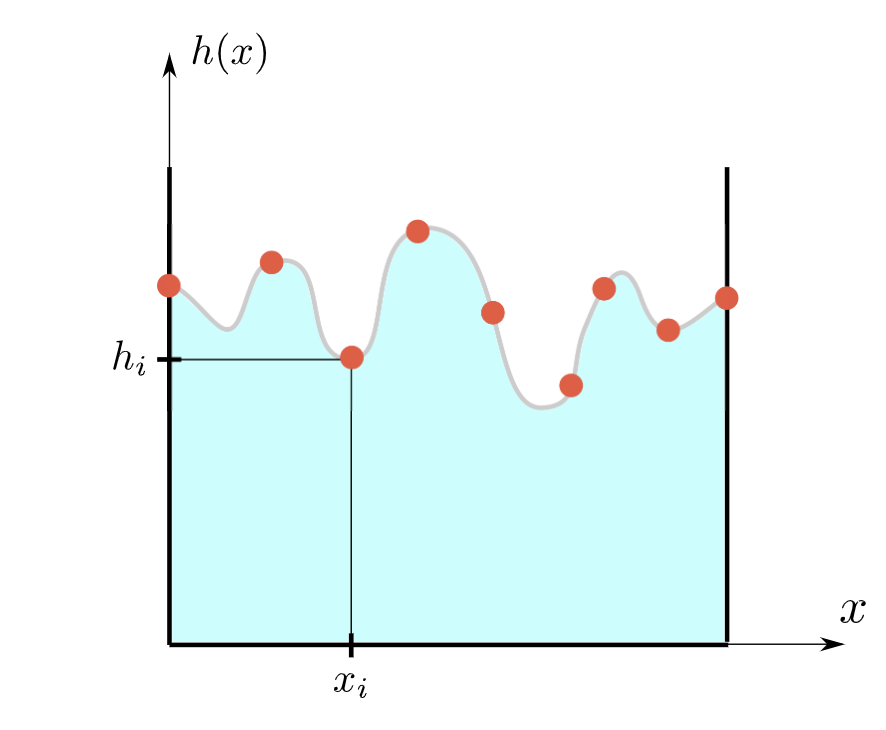
\includegraphics[scale=0.6]{water}}
\caption{Поверхность вязкой жидкости (серая кривая), движущейся сквозь некоторую среду (например, пористую). Её значения известны только в нескольких точках(красные узлы)}
\end{figure}
\begin{figure}[h]
\center{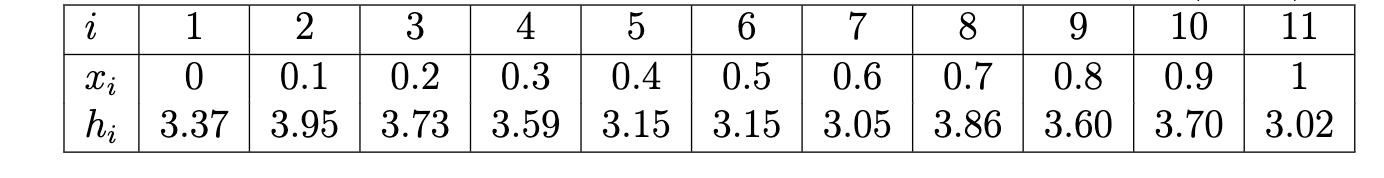
\includegraphics[scale=0.6]{table}}
\caption{Значения уровня поверхности вязкой жидкости}
\end{figure}
\subsubsection*{Продвинутая часть}
\begin{flushleft}
1. Разработать функцию \textit{l_i(i, x, x_nodes)}, которая возвращает значение $i-го$ базисного полинома Лагранжа, заданного на узлах с абсциссами \textit{x_nodes}, в точке  $x$.  \end{flushleft}
\begin{flushleft}
2. Написать функцию \textit{L(x, x_nodes, y_nodes)}, которая возвращает значение интерполяционного полинома Лагранжа, заданного на узлах с абсциссами \textit{x_nodes} и ординатами \textit{y_nodes}, в точке $x$.    
\end{flushleft}
\begin{flushleft}
3. Известно, что при измерении координаты $x_i$ всегда возникает погрешность, которая моделируется случайной величиной с нормальным распределением с нулевым математическим ожиданием и стандартным отклонением $10^{-2}$. Требуется провести следующий анализ, позволяющий выявить влияние этой погрешности на интерполяцию:
\end{flushleft}
\begin{flushleft}
(a) Сгенерировать 1000 векторов значений $[\tilde{x_1}, ..., \tilde{x_{11}}]^T$ , предполагая, что $\tilde{x_i} = x_i + Z$ соответствует значению в таблице 1 и $Z$ является случайной величиной с нормальным распределением с нулевым математическим ожиданием и стандартным отклонением $10^{-2}$.
\end{flushleft}
\begin{flushleft}
(b) Для каждого из полученных векторов построить интерполянт Лагранжа, предполагая, что в качестве абсцисс узлов используются значения $\tilde{x_i}$, а ординат – $h_i$ из таблицы 1. В результате вы должны иметь 1000 различных интерполянтов.
\end{flushleft}
\begin{flushleft}
(c) Предполагая, что все интерполянты представляют собой равновероятные события, построить такие функции $\tilde{h}_l(x) и \tilde{h}_u(x)$, где $\tilde{h}_u(x) < \tilde{h}_u(x)$ для любого $x\in[0;1]$, что вероятность того, что значение интерполянта в точке x будет лежать в интервале [$\tilde{h}_l(x);\tilde{h}_u(x)$] равна 0.9.
\end{flushleft}
\begin{flushleft}
(d) Отобразить на едином графике функции $\tilde{h}_l(x), \tilde{h}_u(x)$ усредненный интерполянт и узлы из таблицы 1.
\end{flushleft}
\begin{flushleft}
(e) Какие участки интерполянта и почему являются наиболее чувствительными к погрешностям?
\end{flushleft}
\begin{flushleft}
4. Повторить анализ, описанный в предыдущем пункте, в предположении, что координаты $x_i$ вам известны точно, в то время как измерения уровня поверхности $h_i$ имеют ту же погрешность, что и в предыдущем пункте. Изменились ли выводы вашего анализа?
\end{flushleft}
\begin{flushleft}
5. Повторить два предыдущие пункта для случая интерполяции кубическим сплайном. Какие выводы вы можете сделать, сравнив результаты анализа для интерполяции Лагранжа и интерполяции кубическим сплайном?
\end{flushleft}
\clearpage
\subsection{Цель выполнения лабораторной работы}

Цель выполнения лабораторной работы -- \GoalOfResearch{}
%----------------------------------------------------------
\subsection{Знакомство с интерполяцией}
\subsubsection{1. Коэффициенты естественного
кубического сплайна}
Разработаем функцию \textit{qubic_spline_coeff(x_nodes, y_nodes)}, которая посредством решения матричного уравнения вычисляет коэффициенты естественного кубического сплайна. Однако, для большего удобства будем возвращать матрицу размерности \\ $(N-1) * 4$, где $N$ - кол-во узлов интерполяции.
Составление и решение матричного уравнения $Ac = b$ и дальнейшее использование коэффицента кубического сплайна $c$ для нахождения других коэффициентов: $a, b, d$ происходит согласно материалу и формулам, предсталенных в лекциях.
\begin{lstlisting}                 
def qubic_spline_coeff(x_nodes, y_nodes):
    N = len(x_nodes)
    A = [[0] * N for i in range (0,N)]
    A[0][0] = 1
    A[N-1][N-1] = 1
    a = [y_nodes[i] for i in range(0, N)]
    h = np.array([x_nodes[i + 1] - x_nodes[i] for i in range(0, N-1)])
    b = np.array([0] + [((3 / h[i] * (a[i + 1] - a[i]) - (3 / h[i - 1] * (a[i] - a[i - 1])))) for i in range (1, N-1)] + [0])
    for i in range (1, N-1):
            A[i][i-1] = h[0]
            A[i][i] = 2*(h[0] + h[1])
            A[i][i+1] = h[1]
    
    A_inv = np.linalg.inv(A)
    c = A_inv @ b
    
    res = np.zeros((N-1 , 4))
    
    for i in range (0, N-1):
        res[i][0] = a[i]
        res[i][1] = ((1 / h[i]) * (a[i+1] - a[i]) - (h[i] / 3) * (c[i+1] + 2*c[i]))
        res[i][2] = c[i]
        res[i][3] = (c[i+1] - c[i]) / (3 * h[i])
    
    return res         
\end{lstlisting}  
\subsubsection{2. Значение кубического сплайна
и его производной в точке}
Напишем функции \textit{qubic_spline(x, qs_coeff)} и \textit{d_qubic_spline(x, qs_coeff)}, которые вычисляют соответственно значение кубического сплайна и его производной в точке $x$ (\textit{qs_coeff} обозначает матрицу коэффициентов).
Аналогично п. 1, формула для кубического сплайна
берется из лекций, формула для производной кубического сплайна получается, соответственно,
посредством дифференцирования формулы для кубического сплайна. \\
$S_i(x_i)  = a_i + b_i(x - x_i) + c_i(x - x_i)^2 + d_i(x - x_i)^3$ - формула кубического сплайна\\
$S_i(x_i)'  = b_i+ 2c_i(x - x_i) + 3d_i(x - x_i)^2$ - формула производной кубического сплайна
\begin{lstlisting}   
def qubic_spline(x_nodes, x, qs_coeff):
  
  for i in range (0, len(x_nodes)-1):
      if (x_nodes [i] <= x <= x_nodes[i+1]):
        k = i
        x_wk = x
        break

  S_i = qs_coeff[k][0] + qs_coeff[k][1] * (x_wk - x_nodes[k]) + qs_coeff[k][2] * ((x_wk - x_nodes[k])**2) + qs_coeff[k][3] * ((x_wk - x_nodes[k])**3)
  return S_i


def d_qubic_spline(x_nodes, x, qs_coeff):
    for i in range (0, len(x_nodes)-1):
      if (x_nodes [i] <= x <= x_nodes[i+1]):
        k = i
        break
        
    Sd_i =  qs_coeff[k][1] + 2 * qs_coeff[k][2] * (x - x_nodes[k]) + 3 * qs_coeff[k][3] * ((x - x_nodes[k])**2)
    return Sd_i
\end{lstlisting} 
\subsubsection{3. График аппроксимации зависимости уровня поверхности жидкости $h(x)$
от координаты $x$}
В данном задании необходимо, используя данные в таблице (Рис. 2), построить аппроксимацию зависимости уровня поверхности жидкости \textit{h(x)} от координаты $x$ с помощью кубического сплайна и продемонстрировать ее на графике вместе с исходными узлами.
Осуществим все это с помощью раннее созданных функций. При этом сгенирируем 1000 точек на отрезке [0;1] с помощью функции бибилиотеки \textit{numpy} языка \textit{Python}.
\begin{lstlisting} 
x = np.linspace(x_nodes[0], x_nodes[10], 1000)
y = [qubic_spline(x_nodes, x[i], res) for i in range (0, len(x))]
plt.subplots(figsize = (10, 10))
plt.plot(x, y, color = 'black')
plt.scatter(x_nodes, y_nodes, color = 'blue', label = 'Интерполяционные узлы')
plt.legend()
plt.grid()
\end{lstlisting} 
\begin{figure}[h]
\center{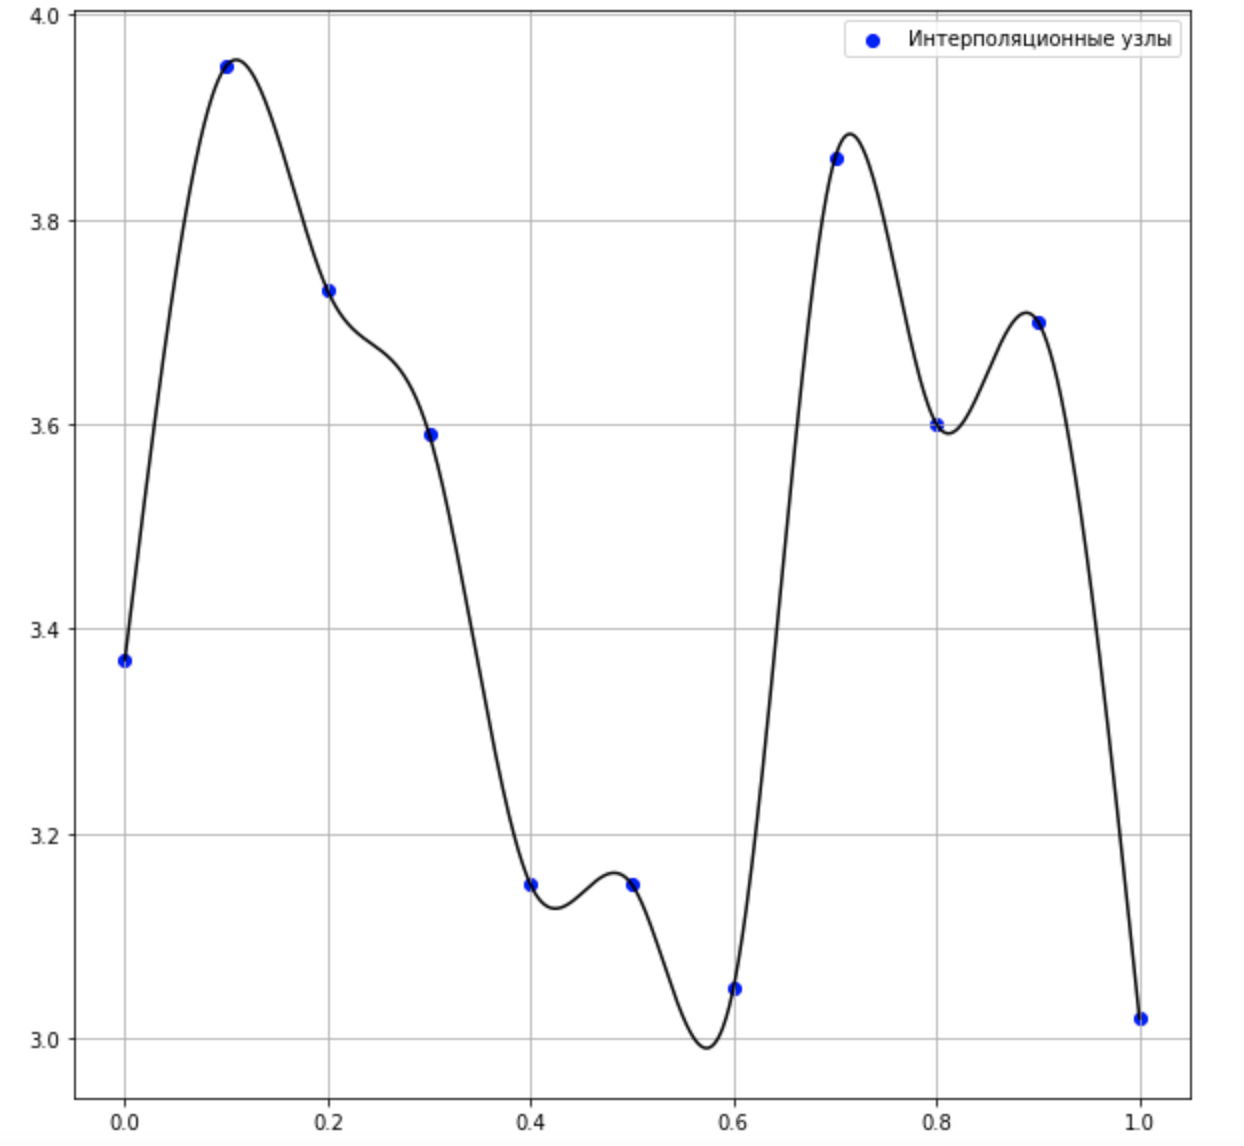
\includegraphics[scale=0.6]{qub_spline_base}}
\caption{Аппроксимация зависимости уровня поверхности жидкости \textit{h(x)} от координаты $x$ с помощью кубического сплайна. Исходные интерполяционные узлы отмечены синим цветом.}
\end{figure}
\clearpage
Для большей наглядности, приложу график производной кубического сплайна, построенного на том же наборе точек, что и график кубического сплайна.
\begin{figure}[h]
\center{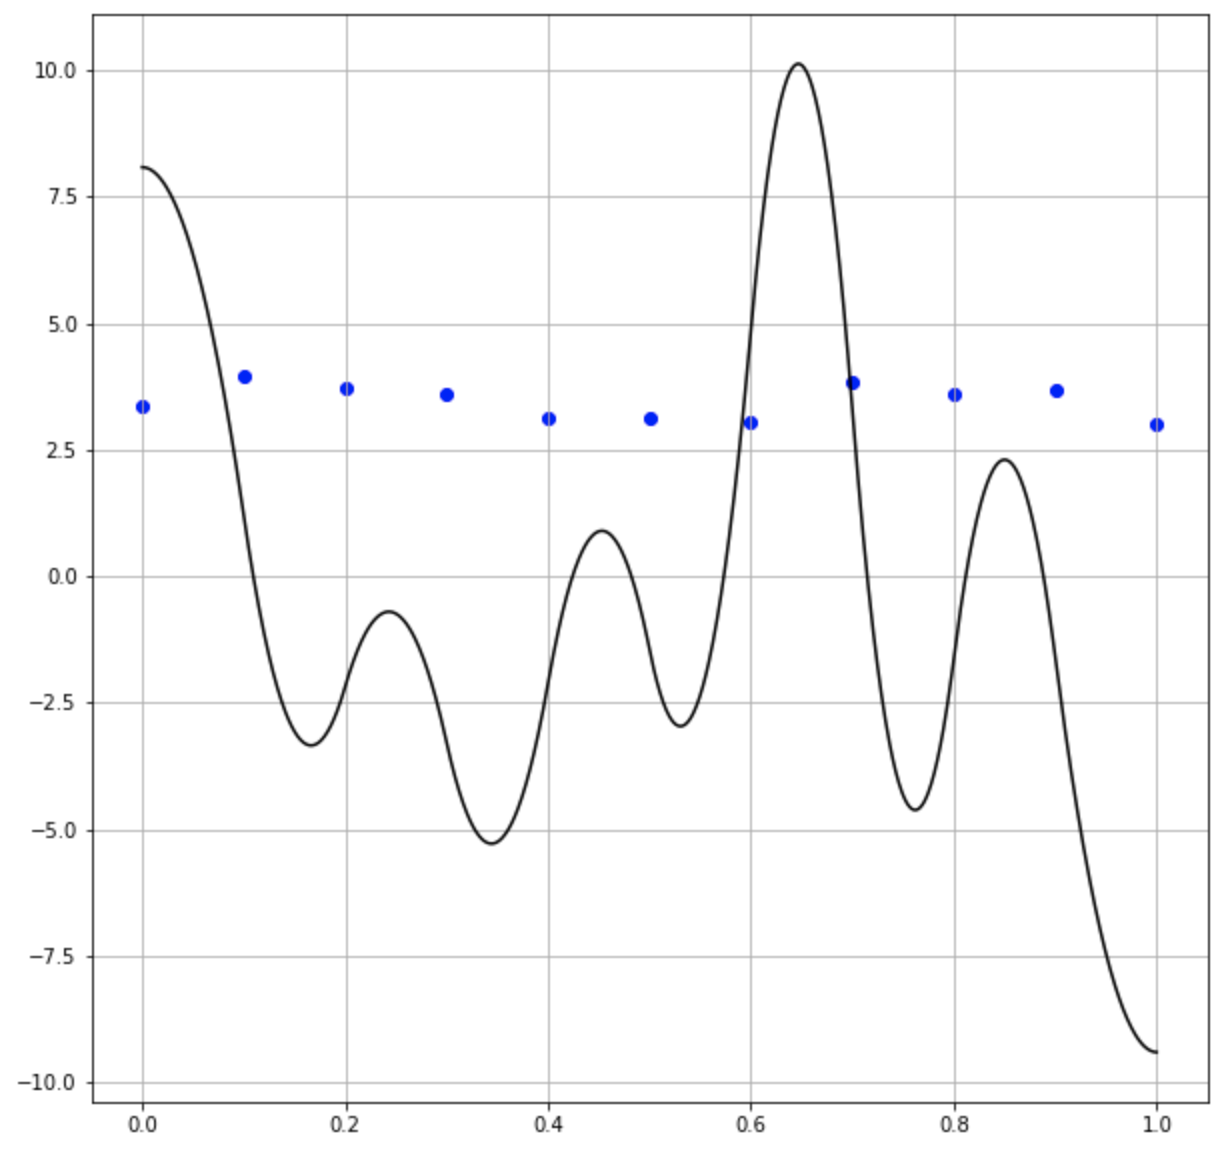
\includegraphics[scale=0.6]{d_qub_spline_base}}
\caption{Производная аппроксимации зависимости уровня поверхности жидкости \textit{h(x)} от координаты $x$ с помощью кубического сплайна. Исходные интерполяционные узлы отмечены синим цветом.}
\end{figure}
%В работе \cite{MIRJALILI201446} авторы пришли к выводу ... $\int_a^{b} f(x)dx$ $\int\limits_a^b f(x)dx$ 
%
%$$
%A_n = \sum\limits_{i=1}^n \frac{a+b}{(c-d)!}
%$$
%
%\begin{equation}\label{direct.task.chem.kinetics}
%\hat{h}_1(x)=(x-x_1){l_1}^2(x)=(x-0)(1-2x)^2=x(1-4x+4x^2)=4x^3-4x^2+x,
%\end{equation}
%
%Формула \{ \} \eqref{direct.task.chem.kinetics} представляет собой базисный полином Эрмита.
%
%\begin{equation}\label{eq.27.eighteen}
%\hat{h_2}(x)=(x-x_2){l_2}^2(x)=(x-\frac12)(2x)^2=(x-1\frac12)4x^2=4x^3-2x^2.
%\end{equation}
%
%Теперь, подставляя полученные выражения (\ref{eq.27.four})-(\ref{eq.27.seven}), (\ref{hermit}), (\ref{eq.27.eighteen}) в выражение (\ref{eq.27.fourteen}), получается следующее выражение:
%\begin{align*}
%H_{3}(x)&=f(x_1)h_1(x)+f(x_2)h_2(x)+f'(x_2)\hat{h_2}(x)+f'(x_2)\hat{h_2}(x)=\\
%&=1\cdot(16x^3-12x^2+1)+e(12x^2-16x^3)+2\cdot(4x^3-4x^2+x) +2e(4x^3-2x^2)=\\
%&=16x^3-12x^2+1+12ex^2-16ex^3+8x^3-8x^2+2x+8ex^3-4ex^2=\\
%&=8x^3(2-2e+1-e)-4x^2(3-3e+2+e)+2x+1=8(3-e)x^3-4(5-2e)x^2+2x+1.\\
%\end{align*}


%----------------------------------------------------------
\clearpage
\subsection{Анализ влияния неопределенностей 
на результат\\ интерполяции}
\subsubsection{1. Базисный полином Лагранжа}

Согласно заданию, разработаем функцию \textit{l_i(i, x, x_nodes)}, которая возвращает значение i-го базисного полинома Лагранжа, заданного на узлах с абсциссами \textit{x_nodes}, в точке $x$. Формула для  $i-го$ базисного полинома Лагранжа представлена в лекциях.
\begin{lstlisting} 
def l_i(i, x, x_nodes):
    num = 1 
    den = 1
    for k in range (0, len(x_nodes)):
        if k == i:
          pass
        else:
          num = num * (x - x_nodes[k])

    for k in range (0, len(x_nodes)):
        if k == i:
          pass
        else:
          den = den * (x_nodes[i] - x_nodes[k])
    l = num / den
    return l
\end{lstlisting} 
\subsubsection{2. Интерполяционный полином Лагранжа }
Согласно заданию, разработаем функцию  \textit{L(x, x_nodes, y_nodes)}, которая возвращает значение интерполяционного полинома Лагранжа, заданного на узлах с абсциссами \textit{x_nodes} и ординатами \textit{y_nodes}, в точке $x$.
Формула для интерполяционного полинома Лагранжа представлена в лекциях.
\begin{lstlisting} 
def L(x, x_nodes, y_nodes):
  L_a = 0
  for i in range (0,len(x_nodes)):
    L_a = L_a + l_i(i, x, x_nodes) * y_nodes[i]
  return L_a
\end{lstlisting} 
%----------------------------------------------------------
\subsubsection{3. Анализ влияния погрешности на интерполяцию (абсциссы узлов)}
\paragraph{a. Генерация 1000 векторов значений $[\tilde{x_1}, ..., \tilde{x_{11}}]^T$ \\} 
\begin{flushleft} Согласно заданию, необходимо: сгенерировать 1000 векторов значений $[\tilde{x_1}, ..., \tilde{x_{11}}]^T$ , предполагая, что $\tilde{x_i} = x_i + Z$ соответствует значению в таблице 1 и $Z$ является случайной величиной с нормальным распределением с нулевым математическим ожиданием и стандартным отклонением $10^{-2}$. \\ Предварительно создадим матрицу необходимой размерности, затем заполним ее, таким образом, что каждый элемент будет иметь вид: 
\textit{vecs[i][j] = x_nodes[j] + np.random.normal(0, 0.01)}
После этого, транспонируем матрицу "иксов"\\с погрешностями, т. к. в условии каждый вектор имеет именно столбец координат узлов по оси абсцисс, а не строку. \\
Библиотечная функция \textit{np.random.normal } модуля \textit{numpy} возвращает образцы нормального распределения, согласно заданным параметрам.
\end{flushleft}
\begin{lstlisting} 
vecs = [[0] * 11 for i in range (0,1000)]
for i in range (0,1000):
  for j in range (0, 11):
    vecs[i][j] = x_nodes[j] + np.random.normal(0, 0.01)
vecs = np.transpose(vecs)
vecs = np.array(vecs)
\end{lstlisting} 
\paragraph{b. Интерполянты Лагранжа для каждого из векторов \\ }
\begin{flushleft}
Необходимо для каждого из раннее полученных векторов (координаты абсцисс с погрешностью, координаты ординат - нет) построить интерполянт Лагранжа. В результате необходимо получить 1000 графиков.
Будем это осуществлять с помощью ранее разработанной функции \textit{L(x, x_nodes, y_nodes)}.
\end{flushleft}
\begin{lstlisting} 
x_int = np.linspace(0, 1, 1000)
interp_lagr = [[L(x_int[i], vecs[: , j], y_nodes) for i in range (0, len(x_int))] for j in range (0, 1000)] 
interp_lagr = np.array(interp_lagr)
plt.subplots(figsize = (10, 10))
for i in range (0, 100):  
  plt.plot(x_int, interp_lagr[i , :])

plt.grid()
\end{lstlisting} 
\clearpage
\begin{figure}[t]
\center{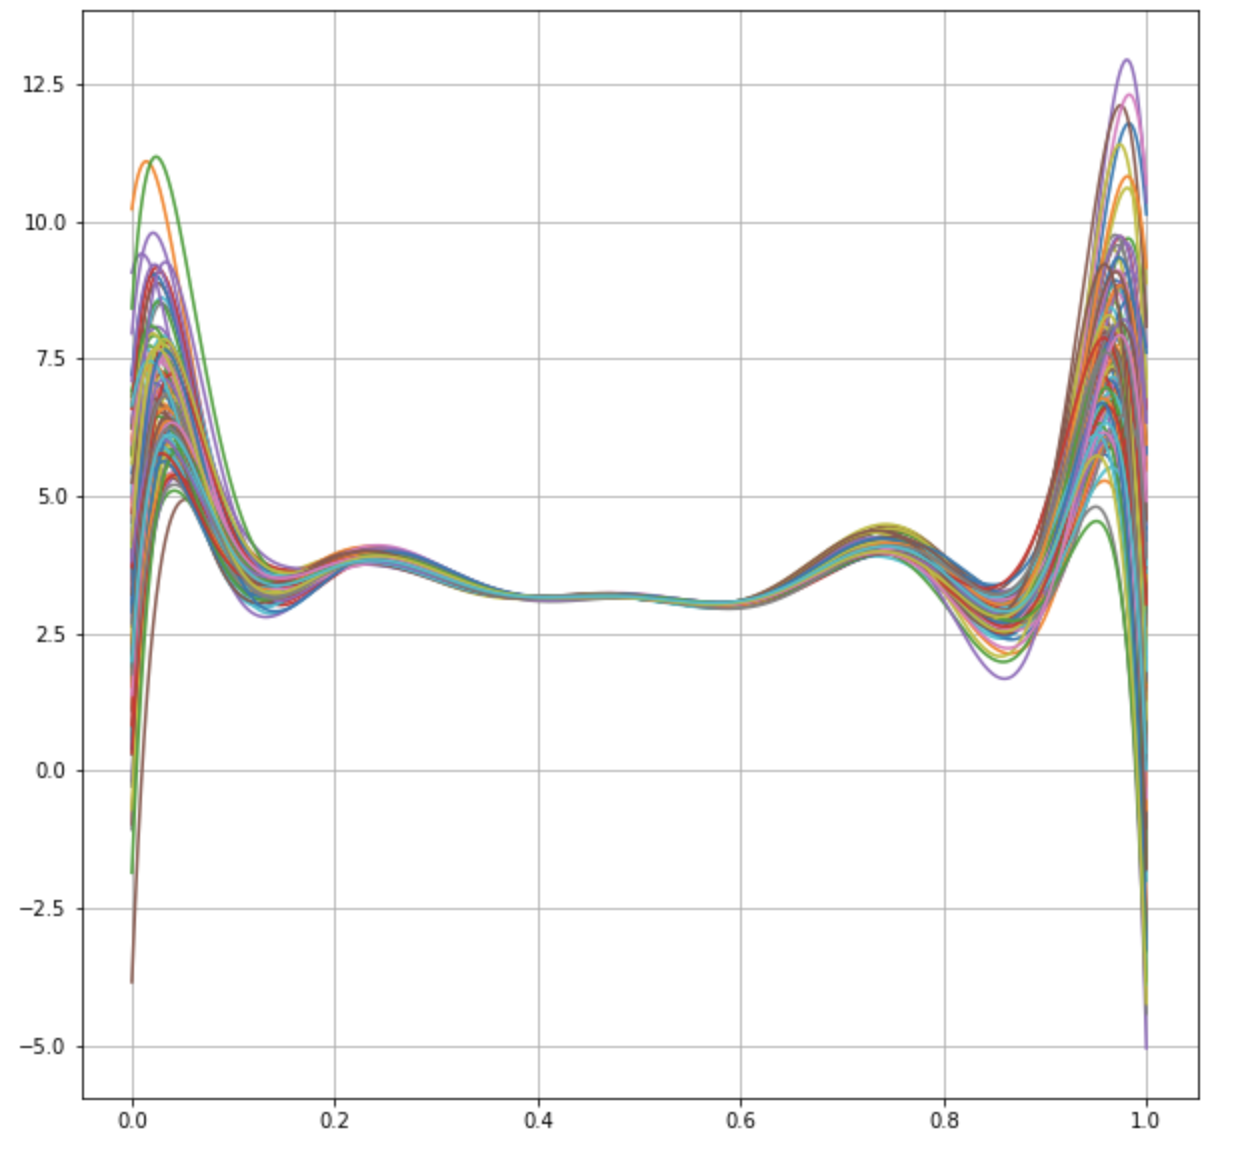
\includegraphics[scale=0.6]{x_lagr}}
\caption{1000 интерполянтов Лагранжа, построенныx на узлах $[\tilde{x_1}, ..., \tilde{x_{11}}]_i$,\textit{y_nodes}}
\end{figure}
\paragraph{c. Построение функций  $\tilde{h}_l(x)$ и $\tilde{h}_u(x)$ (аналитический вид) \\ }
\begin{flushleft}
Необходимо построить функции $\tilde{h}_l(x) и \tilde{h}_u(x)$, где $\tilde{h}_u(x) < \tilde{h}_u(x)$ для любого $x\in[0;1]$, что вероятность того, что значение интерполянта в точке x будет лежать в интервале [$\tilde{h}_l(x);\tilde{h}_u(x)$] равна 0.9.
\\
Осуществим это с помощью функции \textit{percentile} модуля \textit{numpy}.\\
Алгоритм следующий: 
\begin{enumerate}
	\item \textit{Находим срез значений ординат интерполянтов в конкретной точке}
	\item \textit{Находим заданный перцентиль}
	\item \textit{Повторяем для каждой точки}
\end{enumerate}
В итоге получаем набор значений ординат интерполянтов, которые соответствуют заданному перцентилю.
Для решения данной задачи я выбрал перцентиль 5 и, соответственно, 95.
\end{flushleft}
\begin{lstlisting} 
p_95 = [np.percentile(interp_lagr[:, i], 95) for i in range (0, 100)]
p_5 = [np.percentile(interp_lagr[:, i], 5) for i in range (0, 100)]
\end{lstlisting} 
\paragraph{d. Отображение функций  $\tilde{h}_l(x)$ , $\tilde{h}_u(x)$ 
 и усредненного интерполянта, а также интерполяционных узлов\\ }
\begin{flushleft}
Для решения данной задачи, необходимо отобразить
функции  $\tilde{h}_l(x)$ , $\tilde{h}_u(x)$ 
и усредненный интерполянт,и, кроме того, интерполяционные узлы.
Функции $\tilde{h}_l(x)$ , $\tilde{h}_u(x)$ были найдены в прошлом пункте, а усредненный интерполянт находится путем нахождения перцентиля 50. Алгоритм его нахождения аналогичен описанному раннее.
\end{flushleft}
\begin{lstlisting}
mean = [np.percentile(interp_lagr[:, i], 50) for i in range (0, 1000)]
plt.subplots(figsize = (10, 10))
 
plt.plot(x_int, p_95, label = "h_u(x)")
plt.plot(x_int, p_5, label = "h_l(x)")
plt.plot(x_int, mean, label = "Усредненный интерполянт")
plt.scatter(x_nodes, y_nodes, color = 'blue', label = 'Интерполяционные узлы')
plt.legend()
plt.grid()
\end{lstlisting}
\clearpage
\begin{figure}[h]
\center{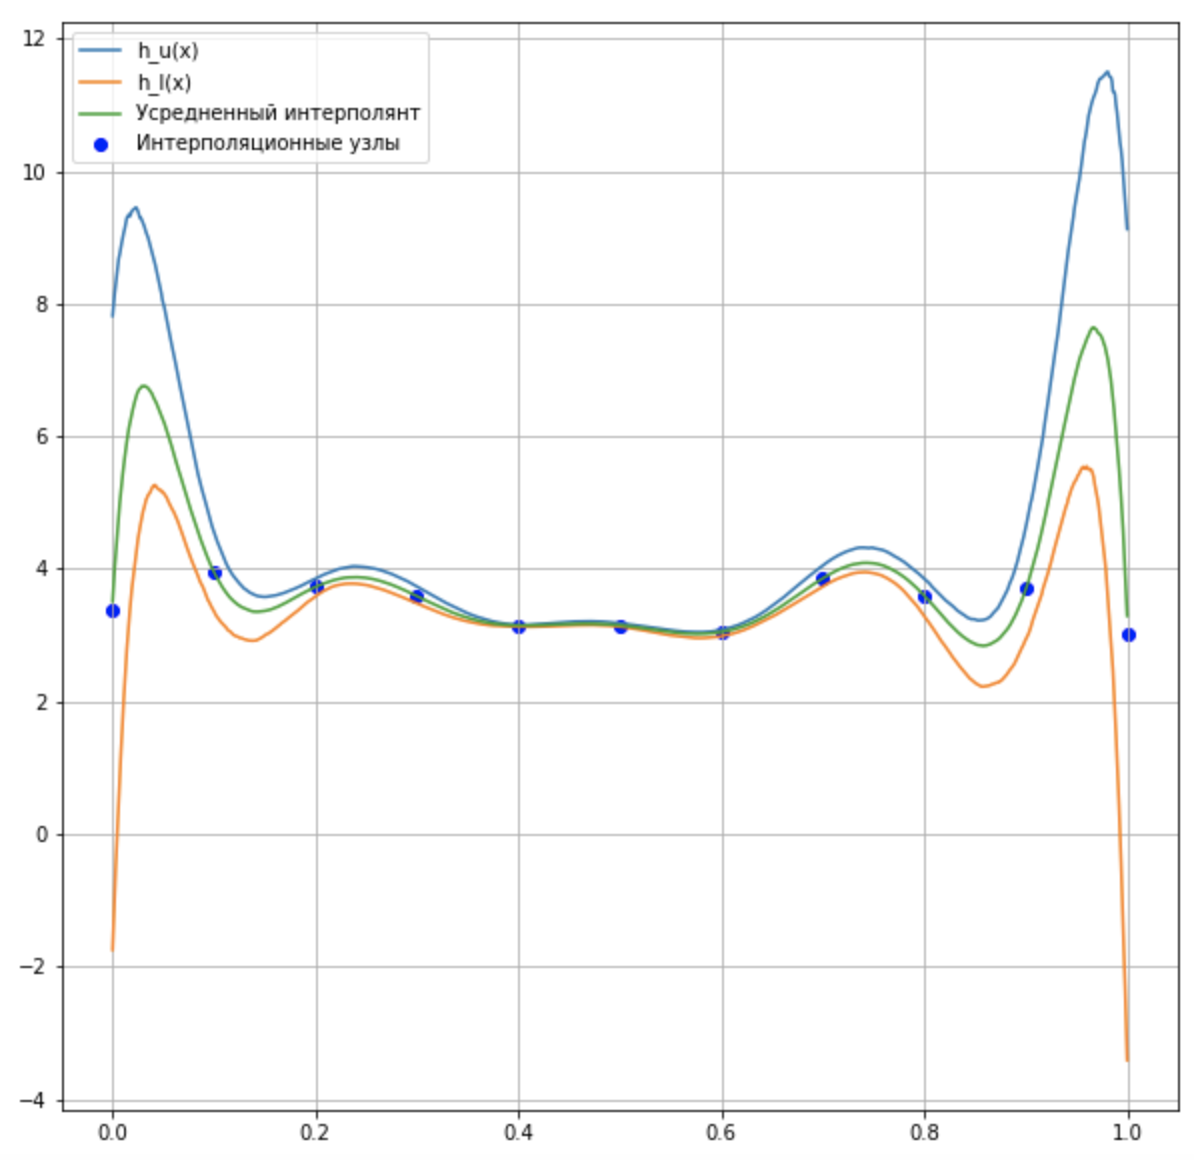
\includegraphics[scale=0.6]{x_lagr_interp}}
\caption{Функции $\tilde{h}_l(x)$ , $\tilde{h}_u(x)$ 
, усредненный интерполянт. Интерполяционные узлы отмечены синим.}
\end{figure}
\paragraph{e. Какие участки интерполянта и почему являются наиболее чувствительными к погрешностям?}
\begin{flushleft}
Паразитные осцилляции, возникающие при интерполяции полиномом Лагранжа, очень сильно проявляются на концах отрезка и слабо в середине.
Проблема такого поведения, заключается в базисных полиномах Лагранжа, именно ближе к концам отрезка интерполирования \textit{"группируются"} их экстремумы. 
Что, собственно, приводит к сильному проявлению паразитных осцилляций.
\end{flushleft}
\subsubsection{4. Анализ влияния погрешности на интерполяцию (ординаты узлов)}
\paragraph{a. Генерация 1000 векторов значений $[\tilde{y_1}, ..., \tilde{y_{11}}]^T$ \\} 
\begin{flushleft}
Пункт выполняется аналогично пункту \textit{3a}
\end{flushleft}
\begin{lstlisting}
vecs1 = [[0] * 11 for i in range (0,1000)]
for i in range (0,1000):
  for j in range (0, 11):
    vecs1[i][j] = y_nodes[j] + np.random.normal(0, 0.01)
vecs1 = np.transpose(vecs1)
vecs1 = np.array(vecs1)
\end{lstlisting}
\paragraph{b. Интерполянты Лагранжа для каждого из векторов \\ }
\begin{flushleft}
Необходимо для каждого из раннее полученных векторов (координаты абсцисс - нет, координаты ординат с погрешностью ) построить интерполянт Лагранжа. В результате необходимо получить 1000 графиков. Решение аналогично
пункту \textit{3b}.
\end{flushleft}
\begin{lstlisting}
x_int = np.linspace(0, 1, 100)
interp_lagr = [[L(x_int[i], x_nodes, vecs1[: , j]) for i in range (0, len(x_int))] for j in range (0, 1000)] 
interp_lagr = np.array(interp_lagr)
plt.subplots(figsize = (10, 10))
for i in range (0, 1000):  
  plt.plot(x_int, interp_lagr[i , :])

plt.grid()
\end{lstlisting}

\begin{figure}[b!]
\center{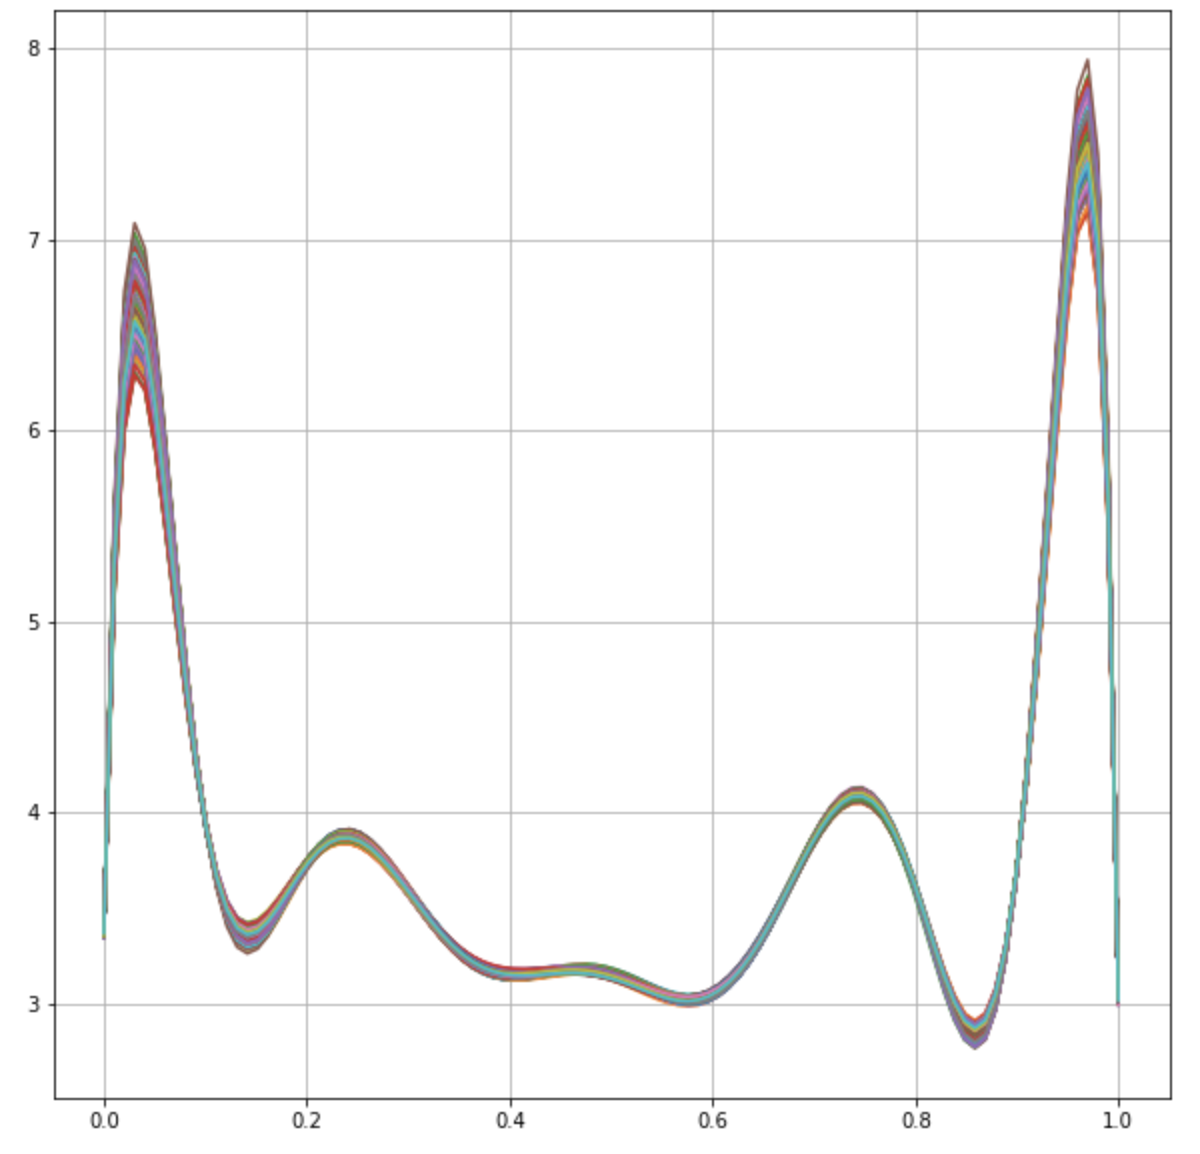
\includegraphics[scale=0.4]{y_lagr}}
\caption{1000 интерполянтов Лагранжа, построенныx на узлах \textit{x_nodes}, $[\tilde{y_1}, ..., \tilde{y_{11}}]_i$ }
\end{figure}
\paragraph{c. Построение функций  $\tilde{h}_l(x)$ и $\tilde{h}_u(x)$ (аналитический вид) \\ }
\begin{flushleft}
Необходимо построить функции $\tilde{h}_l(x) и \tilde{h}_u(x)$, где $\tilde{h}_u(x) < \tilde{h}_u(x)$ для любого $x\in[0;1]$, что вероятность того, что значение интерполянта в точке x будет лежать в интервале [$\tilde{h}_l(x);\tilde{h}_u(x)$] равна 0.9.
\\
Осуществим это с помощью функции \textit{percentile} модуля \textit{numpy}.\\
Алгоритм дальнейшего нахождения данных фукнций совпадает с алгоритмом \textit{3c}
\end{flushleft}
\begin{lstlisting}
p_95 = [np.percentile(interp_lagr[:, i], 95) for i in range (0, 100)]
p_5 = [np.percentile(interp_lagr[:, i], 5) for i in range (0, 100)]
\end{lstlisting}
\paragraph{d. Отображение функций  $\tilde{h}_l(x)$ , $\tilde{h}_u(x)$ 
 и усредненного интерполянта, а также интерполяционных узлов\\ }
\begin{flushleft}
Для решения данной задачи, необходимо отобразить
функции  $\tilde{h}_l(x)$ , $\tilde{h}_u(x)$ 
и усредненный интерполянт, и, кроме того, интерполяционные узлы.
Функции $\tilde{h}_l(x)$ , $\tilde{h}_u(x)$ были найдены в прошлом пункте, а усредненный интерполянт находится путем нахождения перцентиля 50. Алгоритм его нахождения аналогичен описанному раннее.
\end{flushleft}
\begin{lstlisting}
mean = [np.percentile(interp_lagr[:, i], 50) for i in range (0, 100)]
plt.plot(x_int, p_95, label = "h_u(x)")
plt.plot(x_int, p_5, label = "h_l(x)")
plt.plot(x_int, mean, label = "Усредненный интерполянт")
plt.scatter(x_nodes, y_nodes, color = 'blue', label = 'Интерполяционные узлы')
plt.legend()
plt.grid()
\end{lstlisting}
\clearpage
\begin{figure}[h]
\center{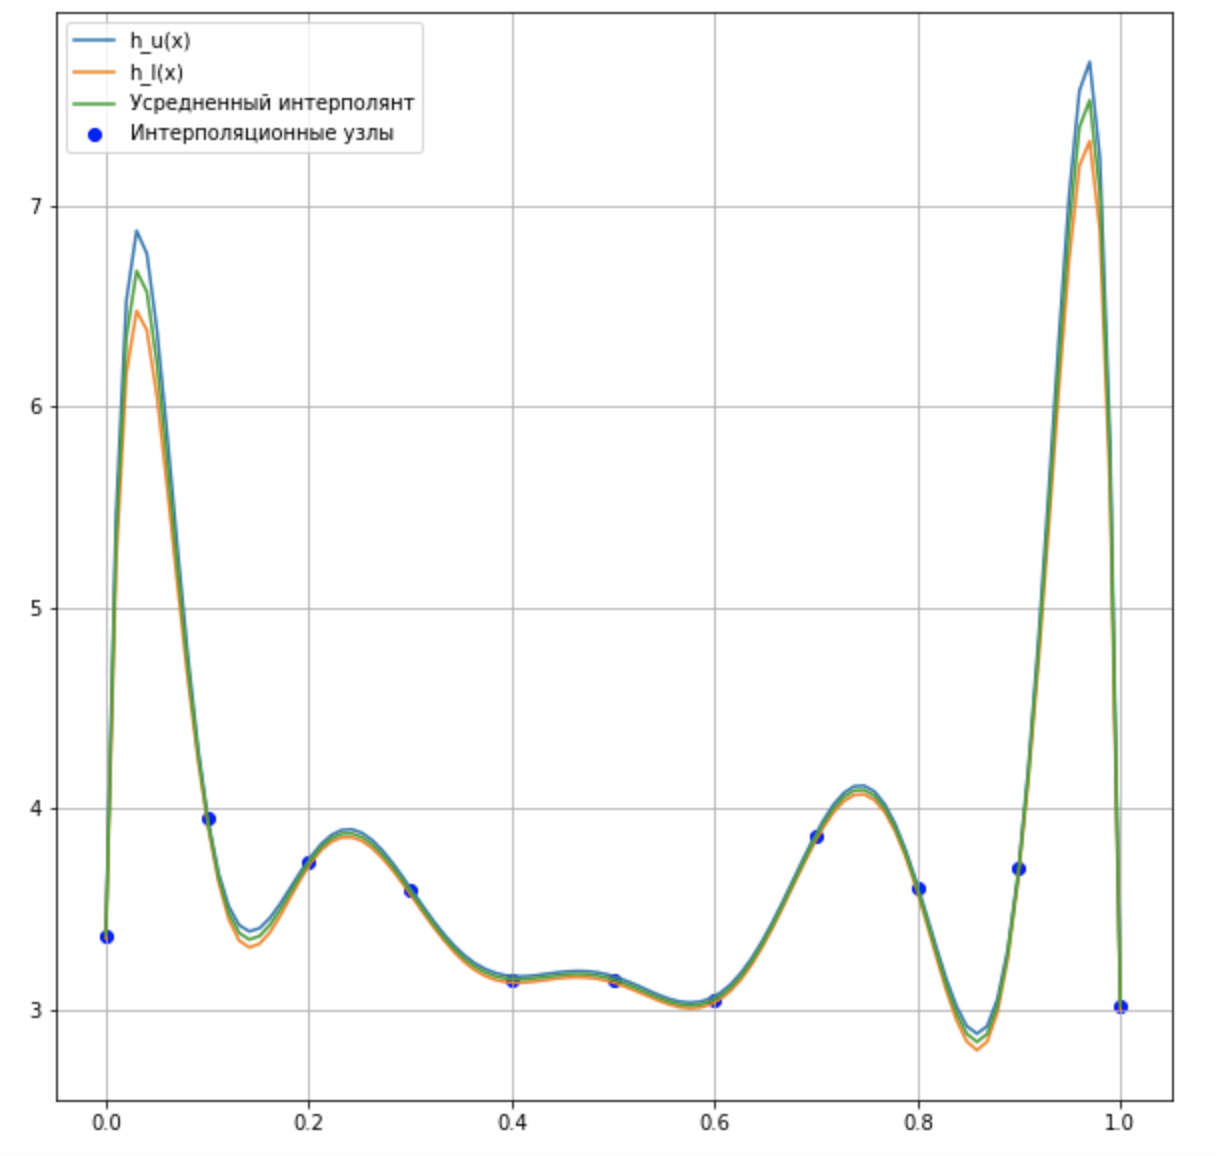
\includegraphics[scale=0.5]{y_lagr_interp}}
\caption{Функции $\tilde{h}_l(x)$ , $\tilde{h}_u(x)$ 
, усредненный интерполянт. Интерполяционные узлы отмечены синим.}
\end{figure}
\paragraph{e. Какие участки интерполянта и почему являются наиболее чувствительными к погрешностям? *Изменились ли выводы вашего анализа? \\}
\begin{flushleft}
Аналогично пункту \textit{3e}, наибольшие паразитные осцилляции наблюдаются ближе к концам отрезка интерполяции. Причина этого - аналогична пункту \textit{3e} и заключается в базисных полиномах Лагранжа. \\
В целом, мои выводы не изменились, однако в данном случае, паразитные осцилляции имеют даже большую видимость, нежели в предыдущем пункте \textit{3e}. Это связано с тем, что значения ординат узлов, на которые умножаются базисные полиномы лагранжа, имееют некоторую погрешность из нормального распределения.
\end{flushleft}
\subsubsection{5. Анализ влияния погрешности на интерполяцию (кубический сплайн)}
\paragraph{1.a. Генерация 1000 векторов значений $[\tilde{x_1}, ..., \tilde{x_{11}}]^T$ \\} 
\begin{flushleft}
Пункт выполняется аналогично пункту \textit{3a}
\end{flushleft}
\begin{lstlisting}
vecs_x_spl = [[0] * 11 for i in range (0,1000)]
for i in range (0,1000):
  for j in range (0, 11):
    vecs_x_spl[i][j] = x_nodes[j] + np.random.normal(0, 0.01) #x_nodes with errors
vecs_x_spl = np.transpose(vecs_x_spl)
vecs_x_spl = np.array(vecs_x_spl)
\end{lstlisting}
\paragraph{1.b. Кубические интерполянты для каждого из векторов \\ }
\begin{flushleft}
Идейно данный пункт совпадает с пунктом \textit{3 b}, однако в данном пункте используется другой способ интерполяции - кубический сплайн.
Кроме того, в контексте данной задачи, необходимо модифицировать функцию \textit{qubic_spline(x, qs_coeff)} и добавить дополнительный аргумент - \textit{x_nodes}, т. к. каждый из сплайнов строится на своем отрезке $[\tilde{x_1}, ..., \tilde{x_{11}}]^T$ 
Кроме того, т. к. потенциально значения $[\tilde{x_1}, ..., \tilde{x_{11}}]^T$ могут располагаться вне отрезка [0;1] или же, не покрывать его полностью, было принято решение в теле функции \textit{qubic_spline(x_nodes, x, qs_coeff)} учесть этот момент и ввести превентивные меры:
\begin{lstlisting}
def qubic_spline(x_nodes, x, qs_coeff):
  x_wk = 0 # if x < x_nodes[0]
  k = 0 # if x < x_nodes[0]
  for i in range (0, len(x_nodes)-1):
      if (x_nodes [i] <= x <= x_nodes[i+1]):
        k = i
        x_wk = x
        break
  if (x>1):
    x_wk = 1 # if x > x_nodes[len(x_nodes) - 1]
    k = len(x_nodes) - 1 # if x > x_nodes[len(x_nodes) - 1]
  S_i = qs_coeff[k][0] + qs_coeff[k][1] * (x_wk - x_nodes[k]) + qs_coeff[k][2] * ((x_wk - x_nodes[k])**2) + qs_coeff[k][3] * ((x_wk - x_nodes[k])**3)
  return S_i
\end{lstlisting}
Алгоритм нахождения значений кубического сплайна в каждой точке:
\end{flushleft}
\begin{enumerate}
	\item \textit{Для каждого сплайна строится своя матрица коэффициентов, по своему набору узлов абсцисс, узлы ординат - общие для каждого сплайна}
	\item \textit{Для каждого сплайна в каждой промежуточной точке отрезка находится свое значение i-го интерполянта}
	\item \textit{После нахождения промежуточных значений для каждого слпайна, строится график, где отображаются все 1000 сплайнов на заданном отрезке}
\end{enumerate}
\begin{lstlisting}
plt.subplots(figsize = (10, 10))

x_nod = np.linspace(x_nodes[0], x_nodes[10], 1000) 
for i in range (0, 1000):

  matrix = qubic_spline_coeff(vecs_x_spl[: , i], y_nodes)
  S = [qubic_spline(vecs_x_spl[: , i], x_nod[j], matrix) for j in range (0, len(x_nod))]
  plt.plot (x, S)

plt.scatter(x_nodes, y_nodes, color = 'blue', label = 'Интерполяционные узлы')
plt.legend()
plt.grid()
\end{lstlisting}
\begin{figure}[h]
\center{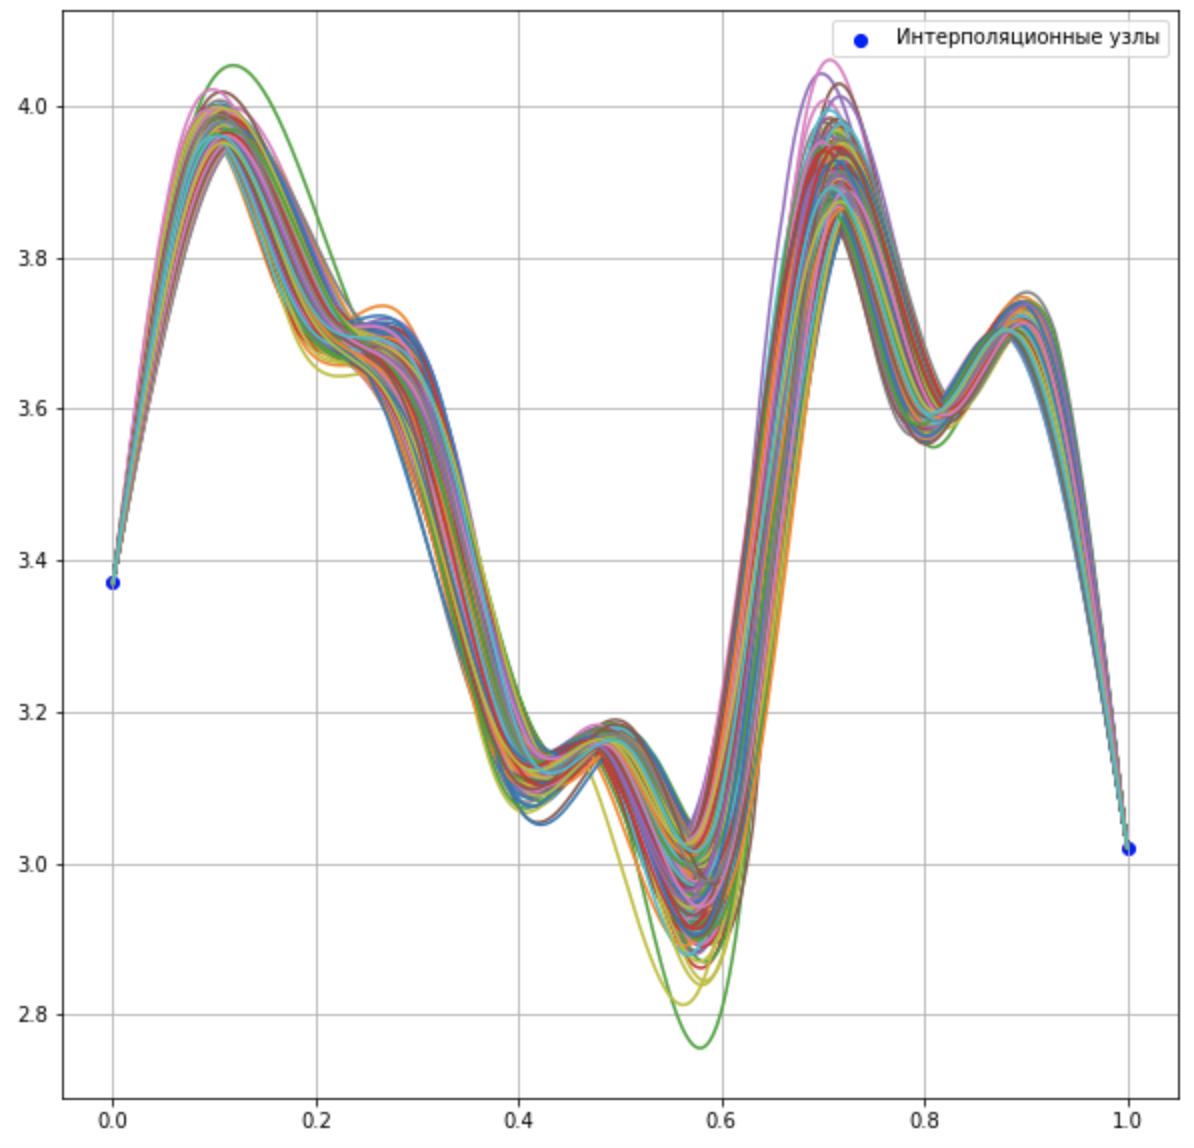
\includegraphics[scale=0.5]{x_spline}}
\caption{1000 графиков для Интерполяции кубическим сплайном, построенныx на узлах $[\tilde{x_1}, ..., \tilde{x_{11}}]_i$, \textit{y_nodes}}
\end{figure}
\paragraph{1.c. Построение функций  $\tilde{h}_l(x)$ и $\tilde{h}_u(x)$ (аналитический вид) \\ }
\begin{flushleft}
Необходимо построить функции $\tilde{h}_l(x) и \tilde{h}_u(x)$, где $\tilde{h}_u(x) < \tilde{h}_u(x)$ для любого $x\in[0;1]$, что вероятность того, что значение интерполянта в точке x будет лежать в интервале [$\tilde{h}_l(x);\tilde{h}_u(x)$] равна 0.9.
\\
Идейно данный пункт схож с пунктом \textit{3.c} (аналогичное использование функции \textit{np.percentile}, однако, т. к. используется другой способ интерполяции, то имеются свои корректировки.
\\
Алгоритм:
\begin{enumerate}
	\item \textit{Создаем пустую матрицу, размерности 1000 x N, где N - кол-во промежуточных точек}
	\item \textit{Для каждого сплайна находим свою матрицу коэффициентов}
	\item \textit{Заполняем матрицу значений сплайна в точке для каждой промежуточной точки и сплайна. В результате получится матрица, содержащая значение каждого сплайна в каждой промежуточной точке}
	\item \textit{Процесс нахождения необходимых значений перцентилей аналогичен пункту 3.с}
\end{enumerate}
\end{flushleft}
\begin{lstlisting}
x_int = np.linspace(0, 1, 1000)
S_res = np.zeros((1000, len(x_int)))
for i in range (0, 1000):
  matrix = qubic_spline_coeff(vecs_x_spl[: , i], y_nodes)
  for j in range (0, len(x_int)):
    S_res[i, j]= qubic_spline(vecs_x_spl[:, i], x_int[j], matrix) 
print(np.shape(S_res))
\end{lstlisting}
\paragraph{1.d. Отображение функций  $\tilde{h}_l(x)$ , $\tilde{h}_u(x)$ 
 и усредненного интерполянта, а также интерполяционных узлов\\ }
\begin{flushleft}
Отобразим на едином графике необходимые функции
\end{flushleft}
\begin{lstlisting}
p_95 = [np.percentile(S_res[:, i], 95) for i in range (0, 1000)]
p_5 = [np.percentile(S_res[:, i], 5) for i in range (0, 1000)]
mean = [np.percentile(S_res[:, i], 50) for i in range (0, 1000)]
plt.subplots(figsize = (10, 10))
 
plt.plot(x_int, p_95)
plt.plot(x_int, p_5)
plt.plot(x_int, mean)
plt.scatter(x_nodes, y_nodes, color = 'blue', label = 'Интерполяционные узлы')
plt.legend()
plt.grid()
\end{lstlisting}
\begin{figure}[h]
\center{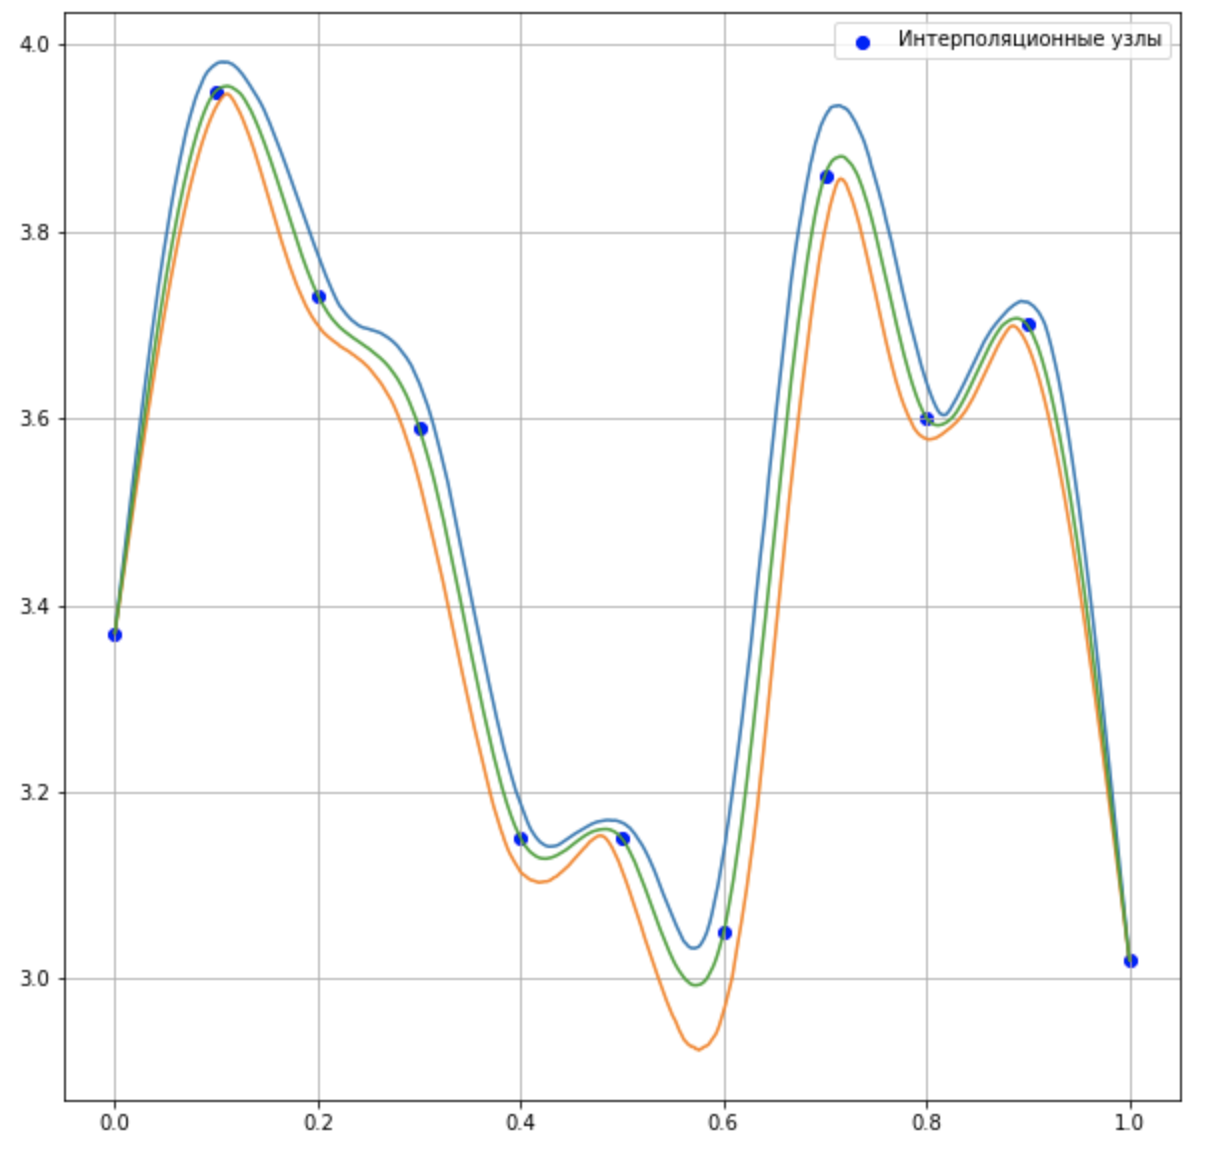
\includegraphics[scale=0.5]{x_spline_interp}}
\caption{Функции $\tilde{h}_l(x)$ , $\tilde{h}_u(x)$ 
, усредненный интерполянт. Интерполяционные узлы отмечены синим.}
\end{figure}
\paragraph{1.e. Какие участки интерполянта и почему являются наиболее чувствительными к погрешностям? *Изменились ли выводы вашего анализа? \\}
\begin{flushleft}
Паразитных осцилляций практически не наблюдается, кроме того, нет тенденции их появления ближе к концам отрезка интерполяции. Причина, почему при интерполяции кубическими сплайнами, паразитных осцилляций меньше чем при интерполяции полиномом Лагранжа, заключается в самом методе аппроксимации - при интерполяции Лагранжа, мы пытаемся аппроксимировать функцию многочленом высокой степени, причем всю функцию сразу. При интерполяции кубическими сплайнами, мы аппроксимируем полиномом заданной степени (не большой, например - в нашем случае: 3) и кроме того, мы аппроксимируем этим полиномом не весь рассматриваемый отрезок, а лишь его часть. То есть вся интерполяция в данном случае получается путем "склеивания" достаточно гладких "кусочков" сплайна, что и приводит к существенно меньшим осцилляциям, ошибкам.
\end{flushleft}
\paragraph{2.a Генерация 1000 векторов значений $[\tilde{y_1}, ..., \tilde{y_{11}}]^T$ \\} 
\begin{flushleft}
Пункт выполняется аналогично пункту \textit{5.1.a}, за тем исключением, что погрешность добавляется не к абсциссам, а к ординатам узлов.
\end{flushleft}
\begin{lstlisting}
vecs_y_spl = [[0] * 11 for i in range (0,1000)]
for i in range (0,1000):
  for j in range (0, 11):
    vecs_y_spl[i][j] = y_nodes[j] + np.random.normal(0, 0.01) #y_nodes with errors 
vecs_y_spl = np.transpose(vecs_y_spl)
vecs_y_spl = np.array(vecs_y_spl)
print(np.shape(vecs_y_spl)
\end{lstlisting}
\paragraph{2.b. Кубические интерполянты для каждого из векторов \\ }
\begin{flushleft}
Пункт аналогичен пункту \textit{5.1.b}.
\end{flushleft}
\begin{lstlisting}
plt.subplots(figsize = (10, 10))

x_nod = np.linspace(x_nodes[0], x_nodes[10], 1000)
for i in range (0, 1000):
  matrix = qubic_spline_coeff(x_nodes, vecs_y_spl[:, i])
  S = [qubic_spline(x_nodes, x_nod[j], matrix) for j in range (0, len(x_nod))]
  plt.plot (x, S)

plt.scatter(x_nodes, y_nodes, color = 'blue', label = 'Интерполяционные узлы')
plt.legend()
plt.grid()
\end{lstlisting}
\clearpage
\begin{figure}[h]
\center{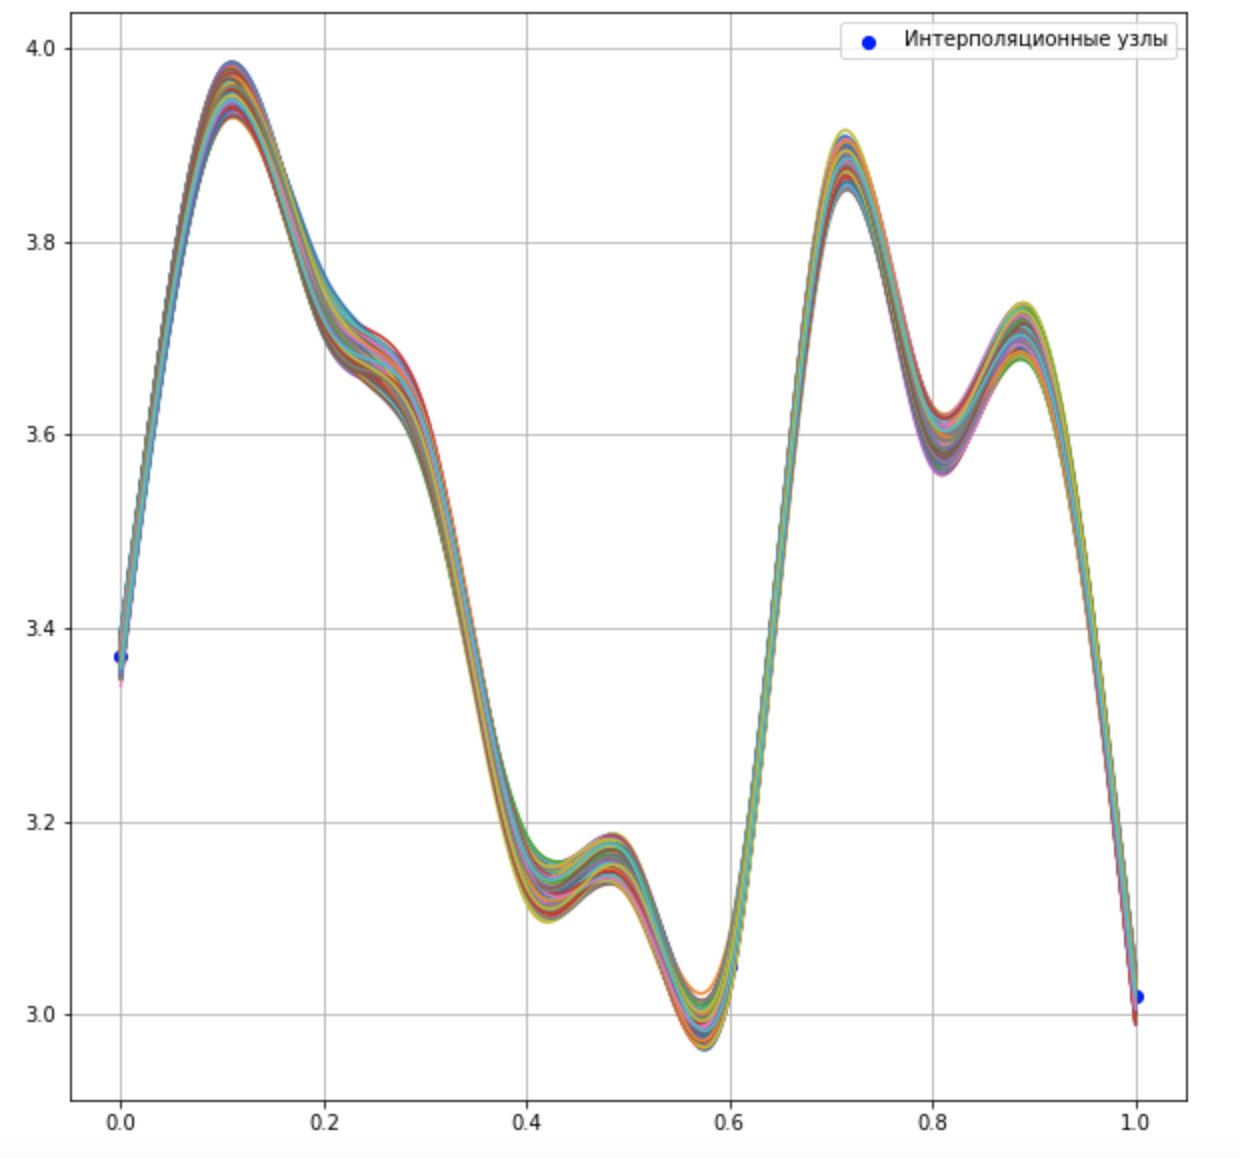
\includegraphics[scale=0.5]{y_spline}}
\caption{1000 графиков для Интерполяции кубическим сплайном, построенныx на узлах \textit(x_nodes), $[\tilde{y_1}, ..., \tilde{y_{11}}]^T$}
\end{figure}
\paragraph{2.c. Построение функций  $\tilde{h}_l(x)$ и $\tilde{h}_u(x)$ (аналитический вид) \\ }
\begin{flushleft}
Пункт аналогичен пункту \textit{5.1.c}. \\
Отличие лишь в том, что в пункте \textit{5.1.c} абсциссы узлов с погрешностями, а в этом пунтке - ординаты узлов с погрешностями.
\end{flushleft}
\begin{lstlisting}
x_int = np.linspace(0, 1, 1000)
S_res1 = np.zeros((1000, len(x_int)))
for i in range (0, 1000):
  matrix = qubic_spline_coeff(x_nodes, vecs_y_spl[:, i])
  for j in range (0, len(x_int)):
    S_res1[i, j] = qubic_spline(x_nodes, x_int[j], matrix)
\end{lstlisting}
\paragraph{2.d. Отображение функций  $\tilde{h}_l(x)$ , $\tilde{h}_u(x)$ 
 и усредненного интерполянта, а также интерполяционных узлов\\ }
\begin{flushleft}
Отобразим на едином графике необходимые функции
\end{flushleft}
\begin{lstlisting}
p_95 = [np.percentile(S_res1[:, i], 95) for i in range (0, 1000)]
p_5 = [np.percentile(S_res1[:, i], 5) for i in range (0, 1000)]
mean = [np.percentile(S_res1[:, i], 50) for i in range (0, 1000)]
plt.subplots(figsize = (10, 10))
 
plt.plot(x_int, p_95)
plt.plot(x_int, p_5)
plt.plot(x_int, mean)
plt.scatter(x_nodes, y_nodes, color = 'red', label = 'Интерполяционные узлы')
plt.legend()
plt.grid()
\end{lstlisting}
\begin{figure}[h]
\center{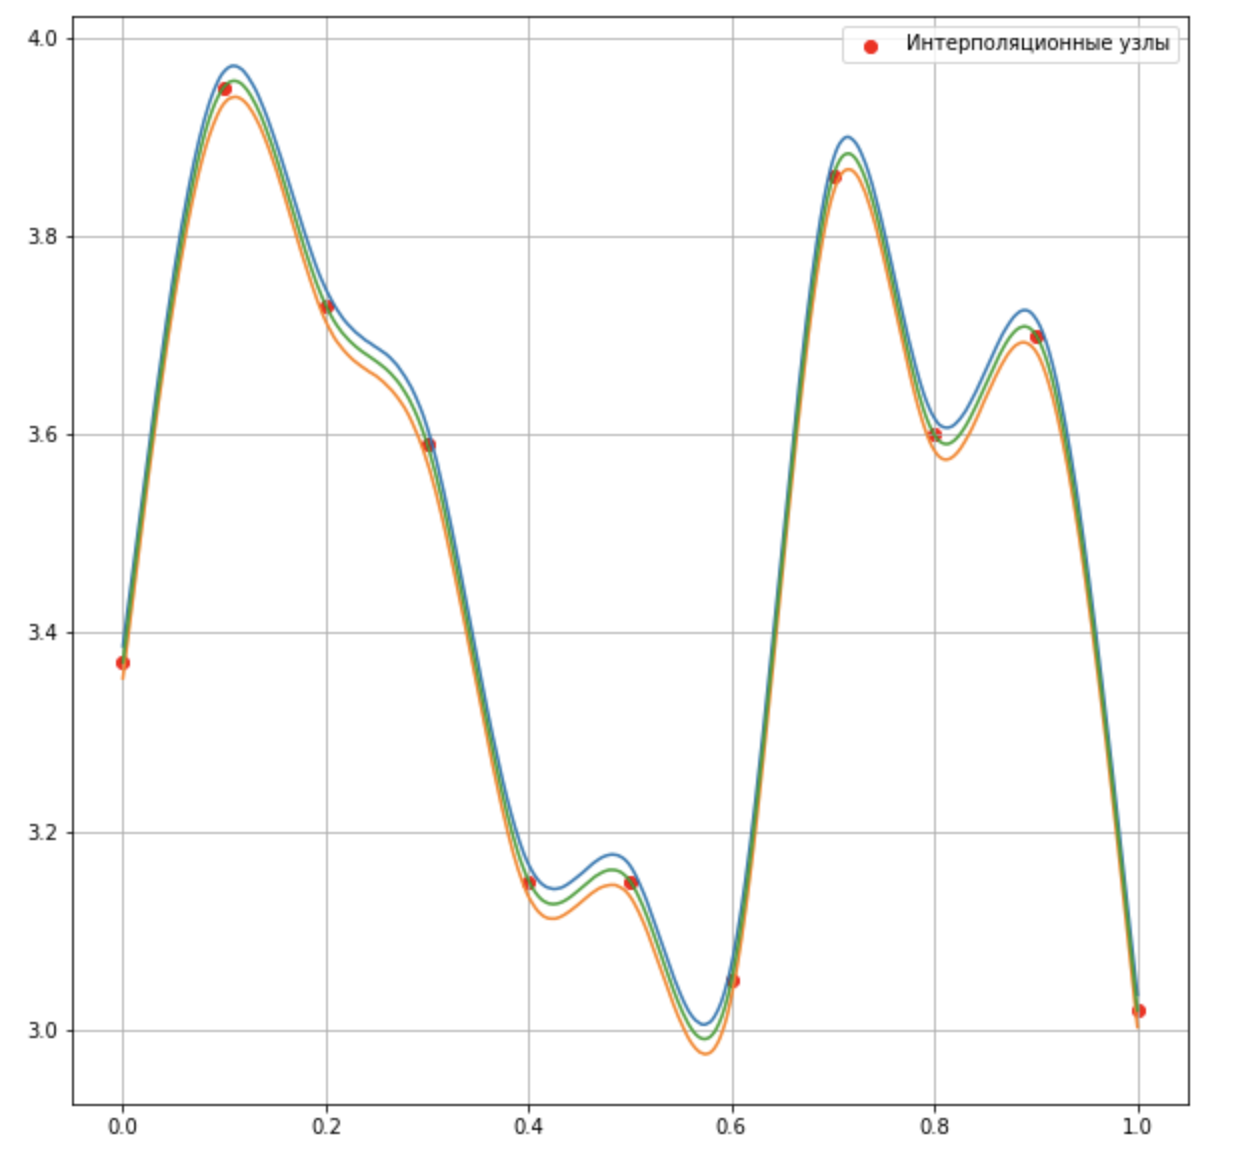
\includegraphics[scale=0.5]{y_spline_interp}}
\caption{Функции $\tilde{h}_l(x)$ , $\tilde{h}_u(x)$ 
, усредненный интерполянт. Интерполяционные узлы отмечены красным.}
\end{figure}
\paragraph{2.e. Какие участки интерполянта и почему являются наиболее чувствительными к погрешностям? *Изменились ли выводы вашего анализа? \\}
\begin{flushleft}
Выводы аналогично пункту \textit{5.1.e}, кроме того, в данном случае паразитных осцилляций еще меньше, что свидельствует о том, что погрешность ординат узлов  менее существенно влияет на итоговую интерполяцию, чем погрешность абсцисс узлов.
\end{flushleft}
\clearpage
\subsection{Заключение}
В ходе данной лабораторной работы было сделано и изучено, а так же проанализировано:
\begin{enumerate}
	\item \textit{Интерполяция в простейшем случае, применение интерполяции к реальным практическим задачам (ассоциация с вязкой жидкостью)}
	\item \textit{Осуществление интерполяции полиномом Лагранжа и кубическими сплайнами}
	\item \textit{Сравнение и анализ одного вида интерполяции при погрешностях разных координат узлов (абсцисс, ординат)}
	\item \textit{Сравнение и анализ разных видов интерполяции при погрешностях разных координат узлов (абсцисс, ординат)}
\end{enumerate}
\begin{flushleft}
В совокупности, данная лабораторная работа позволила лучше проработать материал, связанный с понятиями: аппроксимация, интерполяция, экстраполяция, полином Лагранжа, базисный полином Лагранжа, кубический сплайн, паразитные осцилляции, нормальное распределение, доверительный интервал, перцентиль.
\end{flushleft}
%----------------------------------------------------------
\subsubsection*{Список использованных источников}

\begin{enumerate}
	\item \bibentry{Pershin2018CompMath}
    \item Першин А. Ю. Видео-лекции по курсу "Вычислительная математика". Москва, 2021
    \textit{https://www.youtube.com/channel/UC69GDhPVLY_7IXn3EhmcH2w}
    \item \textrm{[Электронный ресурс]} Wikipedia
    \textit{https://ru.wikipedia.org/wiki/Квантиль}
\end{enumerate}

%----------------------------------------------------------
\subsubsection*{Выходные данные}

\textit{\DocOutReference}
%----------------------------------------------------------
% Атрибуты задачи
\labattributes{}{}{}{}{студент группы \EduGroup, \Author}{\Year, \Semestr}
%----------------------------------------------------------

